\mcchap{Design e sviluppo della soluzione}{cap:designSviluppo}

\section{Origine dei dati}
La principale fonte di dati riguardanti la diffusione della pandemia da COVID-19 in Italia è il Dipartimento della Protezione Civile, che giornalmente a partire dal 24 febbraio pubblica i relativi dati sul repository Github \cite{repository}.

\begin{itemize}
    \item Ricoverati con sintomi: numero di soggetti ricoverati non in terapia intensiva.
    \item Terapia intensiva: Numero di soggetti ricoverati in terapia intensiva.
    \item Totale ospedalizzati: Totale dei soggetti ricoverati in ospedale.
    \item Isolamento domiciliare: Soggetti ricoverati presso la propria abitazione.
    \item Deceduti: Persone decedute positive al virus.
    \item Tamponi: numero di tamponi effettuati (antigenici + molecolari)
\end{itemize}


\begin{figure}[htp]
    \centering
    
\includegraphics[width=5cm]{logo_dpc}
    \caption{Logo del Dipartimento della Protezione Civile}
\end{figure}


\section{Tecnologie utilizzate}

In questo capitolo verranno elencate alcune delle tecnologie utilizzate per lo sviluppo del progetto.

\subsection{Python}
Python è un famoso linguaggio di programmazione ad alto livello, molto utilizzato nel campo \emph{data science}.
Python dispone di librerie e funzioni matematiche integrate, che semplificano il calcolo dei problemi matematici e l'esecuzione dell'analisi dei dati.
\begin{figure}[htp]
    \centering
    
\includegraphics[width=4cm]{python_logo}
    %\caption{Logo di Python}
\end{figure}
Lo sviluppo del progetto è stato svolto interamente in linguaggio Python 3.

\subsection{Plotly}

Plotly è una piattaforma di visualizzazione dati open source dell’omonima azienda che supporta anche grafici interattivi.
Plotly supporta la rappresentazione di svariate tipologie di grafici.
I linguaggi supportati sono Python, R, e Javascript.
\begin{figure}[htp]
    \centering
    
\includegraphics[width=3cm]{plotly_logo}
    %\caption{Logo di Plotly}
\end{figure}

\subsection{Pandas}
Pandas è una libreria Python open source, adatta  per l’analisi e la manipolazione di dati in formato sequenziale o tabellare.
Pandas consente il Caricamento e il salvataggio di formati standard per dati tabellari, come CSV (Comma-separated Values).
Una delle strutture dati utilizzate da Pandas prende il nome di DataFrame, una struttura dati bi-dimensionale, con dimensione variabile che può contenere dati eterogenei.

\subsection{Dash}
La dashboard è stata realizzata utilizzando Dash, un framework Python ideato per costruzione di applicazioni web di analytics.
\noindent Dash si appoggia a Flask, Plotly.sj e react.js. Dash ideale per la costruzione di applicazioni di visualizzazione dati con elevata personalizzazione in puro Python. E’ particolarmente indicato per chiunque lavori con i dati in Python.

\noindent Attraverso alcuni semplici pattern, Dash astrae via tutte le tecnologie e i protocolli necessari che sono richiesti per costruire e interagire con applicazione basate su web.

\subsection{Github}
\noindent GitHub è un servizio web e cloud-based che aiuta gli sviluppatori ad archiviare e gestire il loro codice e a tracciare e controllare le modifiche.

\noindent Git è un sistema che consente il controllo delle versioni e permette sviluppatori di collaborare allo stesso progetto contemporaneamente.
\noindent In sostanza Github, semplifica l’utilizzo del software a riga di comando Git per il controllo delle versioni e la collaborazione.


\begin{figure}[htp]
    \centering
    
\includegraphics[width=3cm]{github_logo}
    \caption{Logo di Github}
\end{figure}

\subsection{Docker}
\noindent Docker è un progetto open source nato con lo scopo di automatizzare la distribuzione di applicazioni sotto forma di “contenitori” detti container.
I container hanno al loro interno tutto il necessario per la corretta esecuzione dell’applicazione, incluse librerie, strumenti di sistema, codice e runtime.

\begin{figure}[htp]
    \centering
    
\includegraphics[width=3cm]{docker_logo}
    \caption{Logo di Docker}
\end{figure}

\noindent Un container è basato su un’immagine che rappresenta tutto il suo contenuto e definisce quale applicativo sarà eseguito al suo interno. 
Per il progetto è stato scelto Docker in quanto consente di isolare una dashboard dalle altre e pertanto semplifica il processo di distribuzione e aggiornamento.

\section{Lo sviluppo}
%% scrivere come è stata sviluppata inizialmente la dashboard

\subsection{Calcoli dei dati}
I calcoli vengono effettuati direttamente nella struttura DataFrame di Pandas
\begin{figure}[htp]
    \centering
    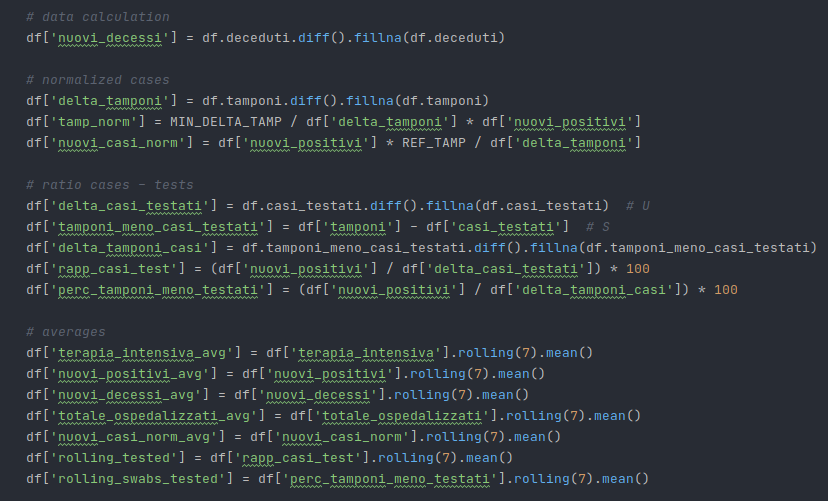
\includegraphics[width=10cm]{data_calculation}
\end{figure}


\subsection{Diagramma di attività}
Un diagramma di attività UML è un diagramma di flusso che rappresenta il flusso del programma da un'attività all'altra,
da un punto iniziale (punto nero pieno) a un punto finale.

\begin{figure}[htp]
    \centering
    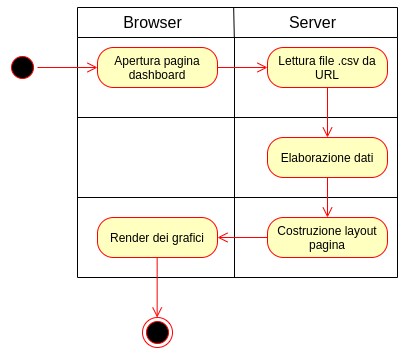
\includegraphics[width=7cm]{activity}
\end{figure}

\subsection{Organizzazione file}
Una applicazione Dash è composta essenzialmente da un singolo programma Python.
Viene utilizzata una versione minimale del framework Bootstrap \footnote{Bootsrap è un framework CSS utilizzato per la semplificare la gestione dello stile della dashboard}, questo assicura dei tempi di caricamento della pagina più rapidi.

\subsubsection{Italia}

\dirtree{%
.1 italy.
.2 assets.
.3 bootstrap.min.css.
.2 dash\_italy.py.
}

\subsubsection{Lombardia}

\dirtree{%
.1 lombardia.
.2 assets.
.3 bootstrap.min.css.
.2 dash\_lombardia.py.
}

\subsubsection{Regioni}

\dirtree{%
.1 lombardia.
.2 assets.
.3 bootstrap.min.css.
.3 img.
.4 Abruzzo.png.
.4 Basilicata.png.
.4 Calabria.png.
.4 ....
.2 dash\_regioni.py.
}



\section{Problemi riscontrati}
I dati forniti dal Dipartimento della Protezione Civile non sono esenti da errori, a causa di errori di trascrizione oppure a causa di comunicazioni parziali o in ritardo dal parte delle regioni.

\noindent Alcune serie di dati, come ad esempio quelli cumulativi come guariti, deceduti, totale casi e tamponi, che dovrebbero essere strettamente crescenti, alcune volte non lo sono.

